\chapter{Implementacija i korisničko sučelje}
		
		
		\section{Korištene tehnologije i alati}
		
			%dio 2. revizije
			
			 %Detaljno navesti sve tehnologije i alate koji su primijenjeni pri izradi dokumentacije i aplikacije. Ukratko ih opisati, te navesti njihovo značenje i mjesto primjene. Za svaki navedeni alat i tehnologiju je potrebno navesti internet poveznicu gdje se mogu preuzeti ili više saznati o njima.
			
			
			\eject 
		
	
		\section{Ispitivanje programskog rješenja}
			
			%dio 2. revizije
			
			 %U ovom poglavlju je potrebno opisati provedbu ispitivanja implementiranih funkcionalnosti na razini komponenti i na razini cijelog sustava s prikazom odabranih ispitnih slučajeva. Studenti trebaju ispitati temeljnu funkcionalnost i rubne uvjete.
	
			
			\subsection{Ispitivanje komponenti}
			%Potrebno je provesti ispitivanje jedinica (engl. unit testing) nad razredima koji implementiraju temeljne funkcionalnosti. Razraditi minimalno 6 ispitnih slučajeva u kojima će se ispitati redovni slučajevi, rubni uvjeti te izazivanje pogreške (engl. exception throwing). Poželjno je stvoriti i ispitni slučaj koji koristi funkcionalnosti koje nisu implementirane. Potrebno je priložiti izvorni kôd svih ispitnih slučajeva te prikaz rezultata izvođenja ispita u razvojnom okruženju (prolaz/pad ispita).
			
			
			
			\subsection{Ispitivanje sustava}
			
			 %Potrebno je provesti i opisati ispitivanje sustava koristeći radni okvir Selenium https://www.seleniumhq.org/ . Razraditi minimalno 4 ispitna slučaja u kojima će se ispitati redovni slučajevi, rubni uvjeti te poziv funkcionalnosti koja nije implementirana/izaziva pogrešku kako bi se vidjelo na koji način sustav reagira kada nešto nije u potpunosti ostvareno. Ispitni slučaj se treba sastojati od ulaza (npr. korisničko ime i lozinka), očekivanog izlaza ili rezultata, koraka ispitivanja i dobivenog izlaza ili rezultata.
			 
			 %Izradu ispitnih slučajeva pomoću radnog okvira Selenium moguće je provesti pomoću jednog od sljedeća dva alata:
			 	%- dodatak za preglednik Selenium IDE - snimanje korisnikovih akcija radi automatskog ponavljanja ispita
			 	%- Selenium WebDriver - podrška za pisanje ispita u jezicima Java, C\#, PHP koristeći posebno programsko sučelje.
	
			\eject 
		
		
		\section{Dijagram razmještaja}
			
			%dio 2. revizije
			
			 %Potrebno je umetnuti specifikacijski dijagram razmještaja i opisati ga. Moguće je umjesto specifikacijskog dijagrama razmještaja umetnuti dijagram razmještaja instanci, pod uvjetom da taj dijagram bolje opisuje neki važniji dio sustava.
			 Dijagrami razmještaja prikazuju konfiguraciju sklopovlja i programske podrške koja se koristi za implementaciju sustava u njegovom operativnom okruženju. Na cloud platformi smješten je poslužitelj baze podataka te web poslužitelji za backend i frontend. Korisnici pristupaju web aplikaciji putem svog web preglednika. Sustav je baziran na arhitekturi "klijent - poslužitelj" s komunikacijom između korisničkih računala(roditelj, pedijatar, doktor, administrator) i poslužitelja putem HTTPS veze.
			\begin{figure}[H]
				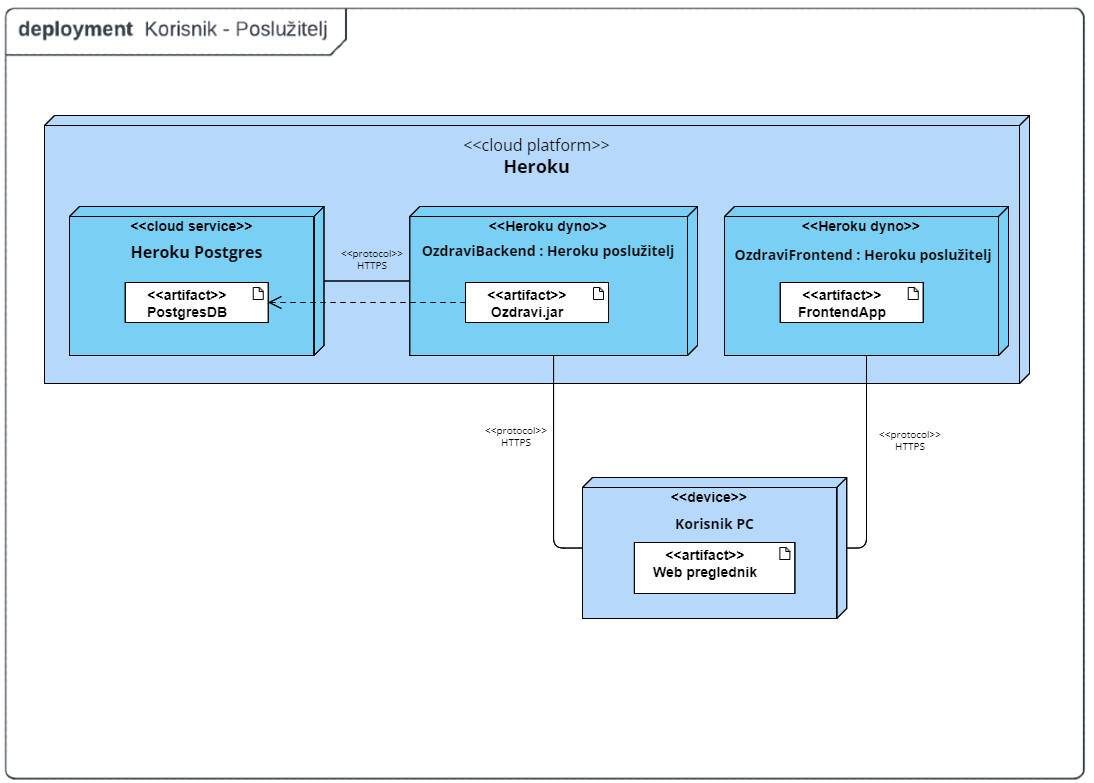
\includegraphics[width=\textwidth]{slike/deploymentDiagram.png} 
				\caption{Dijagram razmještaja} 
			\end{figure}
			\eject 
		
		\section{Upute za puštanje u pogon}
		
			%dio 2. revizije
		
			 %U ovom poglavlju potrebno je dati upute za puštanje u pogon (engl. deployment) ostvarene aplikacije. Na primjer, za web aplikacije, opisati postupak kojim se od izvornog kôda dolazi do potpuno postavljene baze podataka i poslužitelja koji odgovara na upite korisnika. Za mobilnu aplikaciju, postupak kojim se aplikacija izgradi, te postavi na neku od trgovina. Za stolnu (engl. desktop) aplikaciju, postupak kojim se aplikacija instalira na računalo. Ukoliko mobilne i stolne aplikacije komuniciraju s poslužiteljem i/ili bazom podataka, opisati i postupak njihovog postavljanja. Pri izradi uputa preporučuje se naglasiti korake instalacije uporabom natuknica te koristiti što je više moguće slike ekrana kako bi upute bile jasne i jednostavne za slijediti.
			
			
			 %Dovršenu aplikaciju potrebno je pokrenuti na javno dostupnom poslužitelju. Studentima se preporuča korištenje neke od sljedećih besplatnih usluga: https://aws.amazon.com/ {Amazon AWS}, https://azure.microsoft.com/en-us/ Microsoft Azure ili https://www.heroku.com/ Heroku. 
    %Mobilne aplikacije trebaju biti objavljene na F-Droid, Google Play ili Amazon App trgovini.}
	\textbf{Postavljanje baze podataka} \\		
	U procesu postavljanja baze podataka za aplikaciju "Ozdravi", prvi korak je preuzimanje 
	\href{https://www.postgresql.org/download/}{PostgreSQL-a} s ovdje dostupne poveznice za operacijski 
	sustav Windows. Ovaj instalacijski paket obuhvaća PostgreSQL poslužitelj, pgAdmin 
	(grafički alat za upravljanje i razvoj baza podataka) te StackBuilder (upravitelj paketa koji 
	olakšava preuzimanje i instalaciju dodatnih PostgreSQL alata i upravljačkih programa). Nakon završetka 
	instalacije, slijedi standardni postupak postavljanja korisničkog imena i lozinke (neobavezno). \\
	Nakon uspješne instalacije, pokreće se SQL Shell aplikacija.	\\
	
	\begin{figure}[H]
		
\includegraphics[width=\textwidth]{slike/sqlshell1.png} 
		\caption{SQL Shell aplikacija} 
	\end{figure}
	 Kako bi se pristupilo komandnoj liniji, potrebno je pritisnuti tipku Enter dok linija ne započne s \textit{postgres=\#}
	(ako je postavljena lozinka tijekom konfiguracije PostgreSQL-a, onda ju treba unijeti kada sustav zatraži: \textit{Password for user postgres:}). 
	Nakon toga, izvršavaju se sljedeće naredbe:\\
	\textit{create user welebyte with password 'welebyte';\\
	create database ozdravi owner welebyte;}\\
	Sada bi trebala biti stvorena baza podataka "ozdravi", čiji je vlasnik korisnik "welebyte". Naredbom \textit{\textbackslash l} može se provjeriti lista svih postojećih 
	baza podataka i njihovih vlasnika. \\
	\begin{figure}[H]
		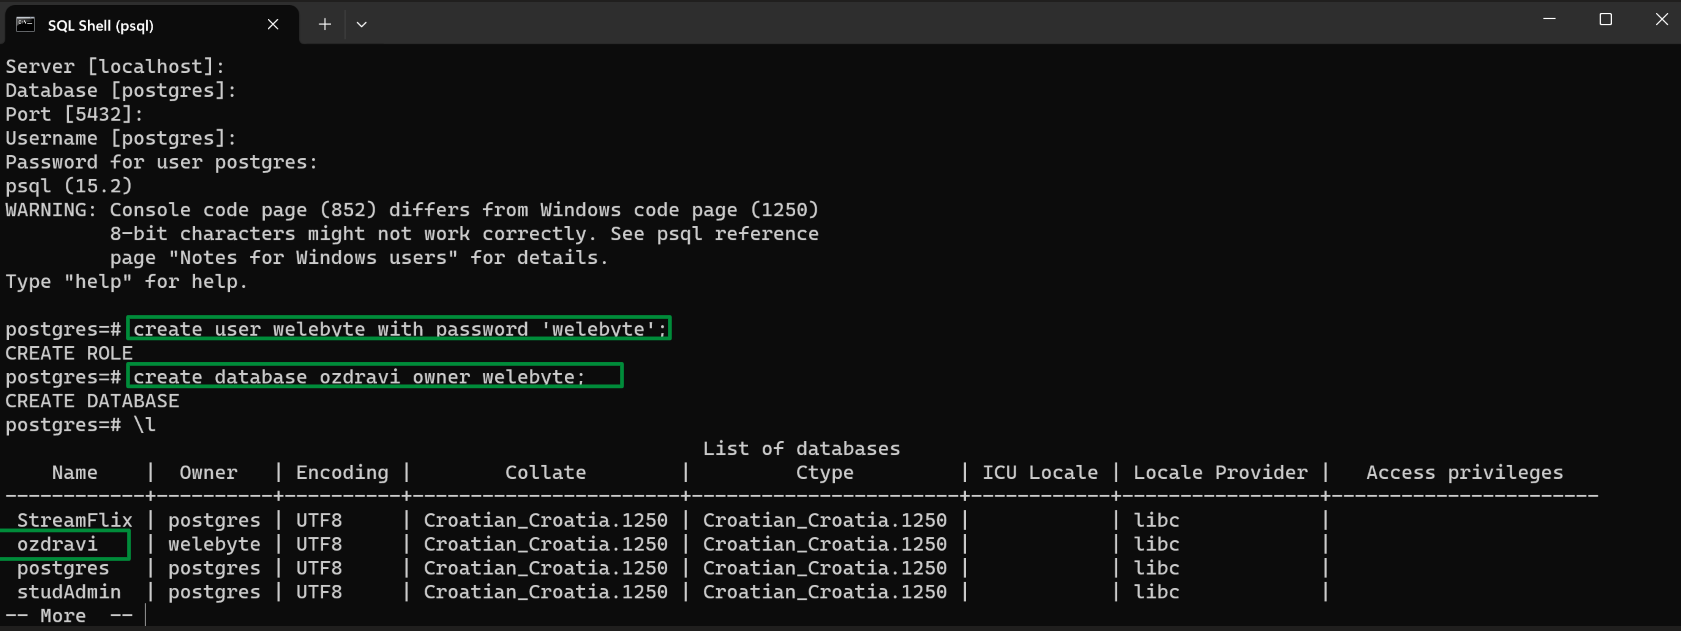
\includegraphics[width=\textwidth]{slike/sqlshell2.png} 
		\caption{Postavljanje baze podataka} 
	\end{figure}
	\noindent\textbf{Pokretanje aplikacije koristeći Intellij} \\
	Nakon uspješne konfiguracije baze podataka, prelazi se na postavljanje aplikacije koristeći IntelliJ IDE. Potrebno je otvoriti mapu \textit{IzvorniKod\textbackslash ozdravi-backend} kao 
	novi projekt u IntelliJ-u, a aplikacija se dalje pokreće jednostavnim pokretanjem datoteke \textit{OzdraviBackendApplication.java}. Aplikacija je sada dostupna na adresi:
	\url{http://localhost:8000}.\\
	\\
	\textbf{Postavljanje frontenda}\\
	Sljedeći korak uključuje postavljanje frontenda. Prvotno se preuzima okruženje za izvršavanje JavaScript koda, Node.js, s ovdje dostupne 
	\href{https://nodejs.org/en/download/}{poveznice}, slijedeći standardne korake instalacije. Zatim, u naredbenom retku (terminalu), potrebno se pozicionirati 
	u direktorij u kojem je spremljen izvorni kod za frontend: \textit{...IzvorniKod\textbackslash ozdravi-frontend}. Prilikom prvog pokretanja, izvršava se naredba \textit{npm install} kako bi se 
	preuzeli svi potrebni paketi, a zatim se aplikacija pokreće naredbom \textit{npm start}.
	\begin{figure}[H]
		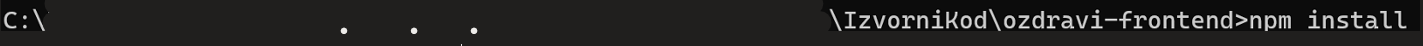
\includegraphics[width=\textwidth]{slike/npmin.png} 
		\caption{Preuzimanje paketa} 
	\end{figure}
	\begin{figure}[H]
		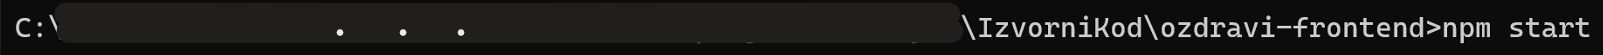
\includegraphics[width=\textwidth]{slike/npmst.png} 
		\caption{Pokretanje aplikacije} 
	\end{figure}
	
	\newpage \noindent Nakon pokretanja, aplikaciju je moguće vidjeti na adresi: \url{http://localhost:3000.}\\
	\begin{figure}[H]
		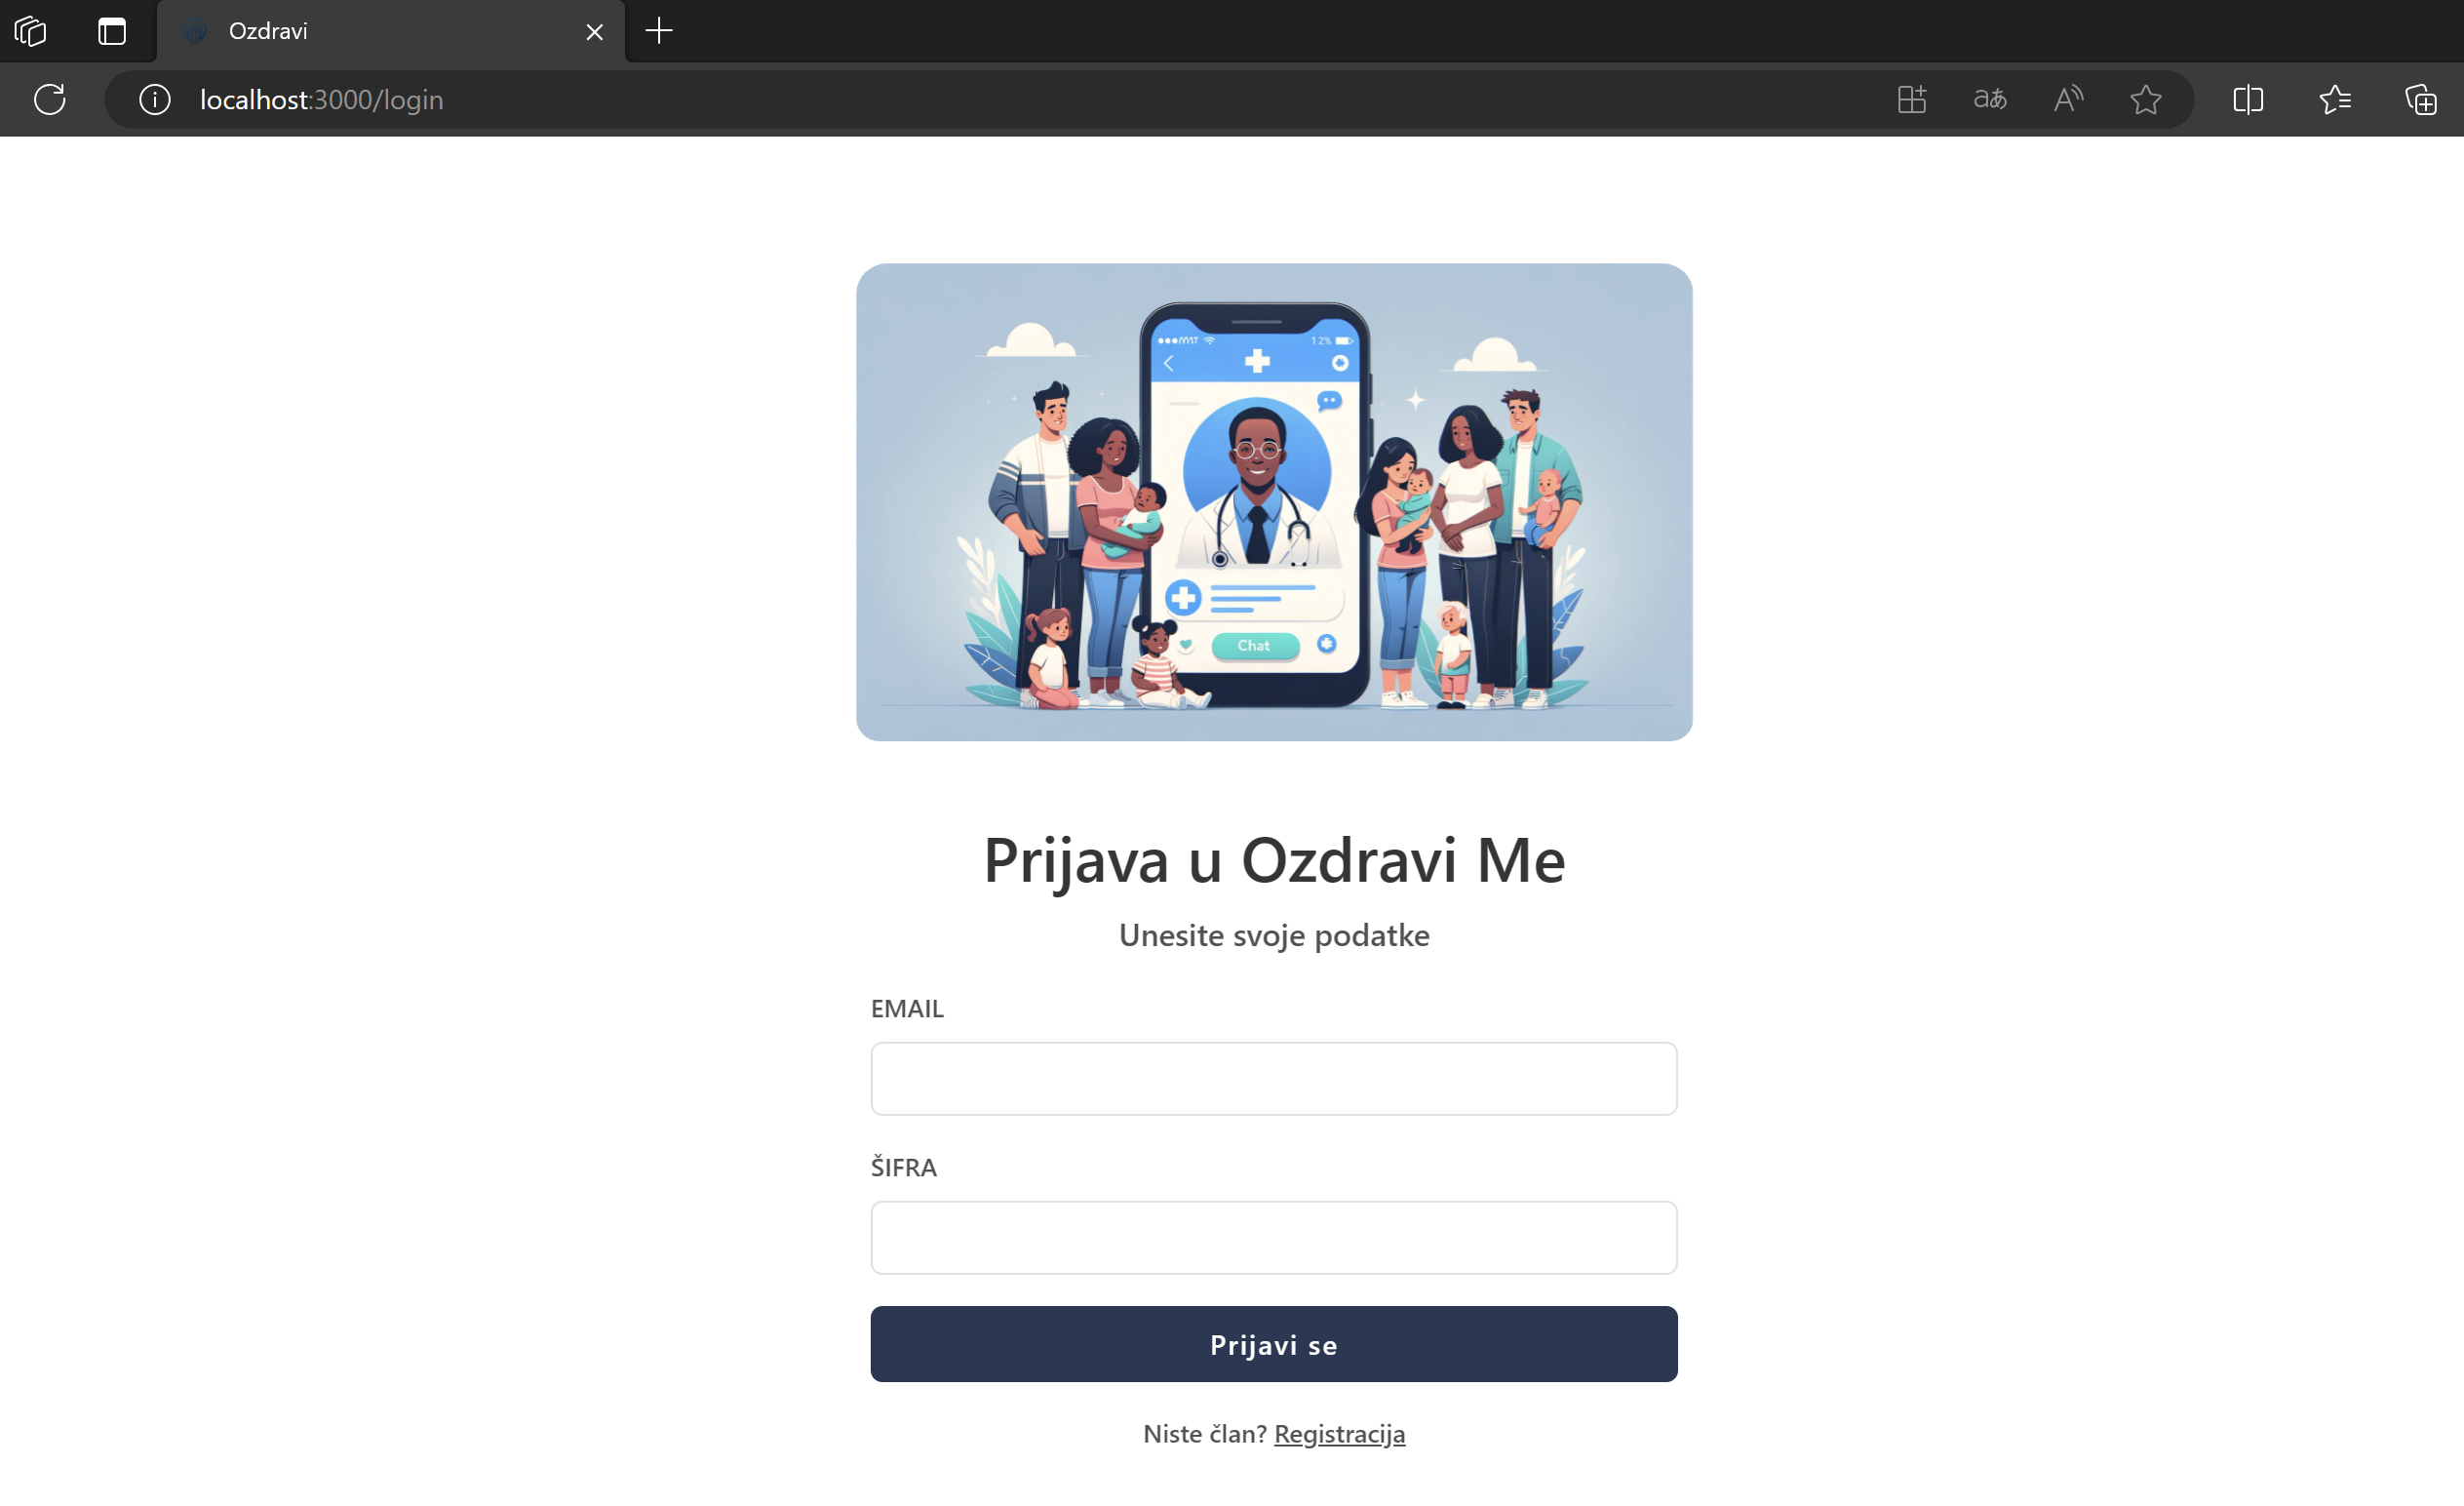
\includegraphics[width=\textwidth]{slike/loc3000.png} 
		\caption{Aplikacija na portu 3000} 
	   \end{figure}
	Nakon svake promjene i spremanja koda, stranica se automatski ponovno učitava. Osim toga, postoji mogućnost promjene porta aplikacije uređivanjem datoteke 
	\textit{package.json}, 
	gdje se u liniji koda 
	\textit{"start": set PORT=3006 \&\& react-scripts start} može izmijeniti broj porta prema želji.
	\eject 